\section{Introduction}
\label{sec:intro}

Substantial research effort in robot planning has revolved around how
plans are executed and how threats to robust execution can be dealt
with in-situ \kcomment{citations needed}. This is particularly
important in dynamic and unpredictable real-world environments where
plans can and do change rapidly and the robotic agent is expected to
be responsive to such exogenous change. Often this focus has been
driven by the need to replan given a priori goals. It is often assumed
in such systems, that goals or objectives are known a priori with the
agent having to deal with the dynamism associated at the execution end
of the system. 

In this paper, we argue that the impact of asynchronous arrival of
goals and their consequent impact on execution is important to
understand for the agent to systematically deal with a dynamic
environment, and one that has been less well studied. We emphasize the
need for planning and plan execution in-situ to enable tight closure
of control loops for the robot's responsiveness.
% In order for an agent to operate in a dynamic environment, the agent
% needs to be constantly observing the external world so that it can
% keep up to date with how the world is changing. Therefore, a robotic
% agent needs to be planning in situ so that it can alter, or update,
% its plan according to the changes. The actual execution of the plan
% will also need to change accordingly. The execution also provide
% constant feedback on how the world is evolving.  Thus as a result of
% the dynamic environment, the robotic agent will need to anticipate
% constant changes in the plan and need to evaluate how to properly
% execute the plan.
The ability to plan in-situ leverages the ability to dynamically add
new objectives to the agent during mission execution instead of being
forced to specify them beforehand.  While such capabilities allow for
more flexible and autonomous missions it also makes the overall misson
execution more challenging.

In the pursuit of planning in a dynamic environment, earlier work done
in \texttt{IPEM} \cite{AmbrosIngerson88}, \texttt{ROGUE}
\cite{Haigh98}, and the LAAS Architecture \cite{alami:1998p820} have
all helped to make real-world planning possible. Based on these past
successes, there have been multiple experiments that have successfully
functioned in the real-world, the Remote Agent Experiment \texttt{RAX}
\cite{mus98}, the Autonomous Spacecraft Experiment \texttt{ASE}
\cite{chien99} and more recently the Teleo Reactive Execution \rxe
\cite{mcgann08b,py10}. In all these systems, generative plans are
dispatched for execution using rich representations that deal with
durative actions and resources \cite{lemai04}, the focus of our work
here.

In particular, our focus is on constraint-based temporal planning
\cite{frank2003} with a demonstrated capability for real-world
planning and execution.
% Most of these modern systems are using at the high-level 
% constraint-based planner with rich representation of resources 
% and time such as the ones presented in \cite{frank2003,lemai04}. 
They often implement least-commitment planning generating a solution
that does not commit to specific values (\eg action start and end
times) unless explicitly required by the model. Such flexibility puts
the burden on the plan executive to decide at which time a specific
action within all possible values, can be dispatched. 
% Resolving this problem resulted on a large amount of research both
% considering how to represent the plan to be dispatched to the
% executive with a compact yet complete representation, along with more
% refinements on how to deal with uncontrollable constraints. Still,
The challenge of deciding whether the next possible set of action(s)
should be started immediately or if it should be postponed for a later
start date.

Procrastination is avoided by starting actions as early as possible
while ensuring that it does not impact plan brittleness. This choice
is lead by the intuition that by starting actions early it gives more
room in the future to deal with worst case execution scenarios. While
this solution works in the general case where all the goals of the
agent are known a priori, it is challenging when the agent can have
new objectives added during the course of mission execution and leads
to the typical dichotomy of dealing with \emph{when} to start an
activity. Dispatching actions too early can lead can lead the agent to
premature commitment towards a course of action dictated by the plan
which can change in a dynamic context; waiting inordinately on the
other hand, could either lead to doing nothing in the interim or
missing the ability to deal with opportunistic events.
% the agent in a
% situation where the new goal received is not integrated as efficiently
% as it would have been should the agent have waited before taking
% action.
In this context, it is important for the agent make a distinction
between actions that can be taken proactively versus other actions
that may not be urgent.  

In this work, we propose a systematic approach to allow the agent to
make such distinction for each action by tracing the causal relations
with goals within the current plan.  This allow us to determine the
best dispatch strategy based on the nature of the goals this action
contributes to.

% \fcomment{Plan for the paper here}
The structure of this paper is as follow. We introduce an example
illustrating the problem of a flexible plan execution. We then discuss
previous works and how they do tend to focus on a single policy or not
consider the possibile emergence of new goal during the mission. We
then present algorithmic solutions that allow to decide at execution
when actions should be started. Finally after presenting the results
we obtain on our implementation we conclude and present further
research that need to be addressed.



% this can have a
% negative impact when consider that new goals for the agent could
% emerge as it execute its mission.

	
% \fcomment{I need to rework the following section, started here}
% At the highest level of abstraction, constraint-based temporal
% planning uses a temporal plan to organize how the world works. A
% temporal plan is made up of multiple timelines which each describe the
% evolution of a subsystem in chronological order. An example of a
% subsystem would be the navigator for a robotic agent. Each timeline is
% simply the encapsulation of all the possible state values for a
% subsystem, within the parameters of a plan.  Therefore, a timeline can
% be broken down into its state values along with their temporal
% extents, which are defined as tokens. As the base unit for a timeline,
% tokens describe the simplest behavior of a subsystem e.g. turn
% right. THis kind of representation as it follows least commitment
% planning strategy. It herefore allow to have a plan which is partailly
% grounded and especially tokens star, duration anfd end times are
% represented as intervals depiciting all the acceptable values for
% each. By doing so this leave  mroe flexiblity during execution to
% decided when -- within the specified domains -- an event should
% occur accroding to the current context. This also raises the probelem
% that thids decision should then be taken after the plan was produced
% by the executive. A lot of exitiing work ahas been made in the area on
% the best approach to send the plan to dispach the produced plan to an
% executive so it is easier for it to maintin the temporla constraints
% within this plan at execution (references). This still leave an issue
% open : how does one decide at execution whether a plan actitivy (or
% token) should be started as soon as possible or can be postponed
% later. This problem can become imporatnt when you see the plan being
% produced within a situated agent. Indeed, while the current set of
% objectives fr the agent is known these can evolve as time advance and
% the poperators or other agents give it new objectives to be
% fullfilled.
% It becomes therefore important for the agent to be
% proactive when required while being able to disitinguish actions that
% are not yet urgent.
% It is understood that grounding the start and end times of a
% token decrease the robustness of a robotic agent while in a dynamic
% environment (citations). Therefore, the tokens have flexible intervals
% for their start, duration, and end times.  As an example, the turn
% right behavior could start from a lower bound time of 12pm to an upper
% bound time of 3pm. This means it can start anytime between its lower
% and upper bound, keeping it flexible.  Consequently, it is the agents
% task to choose exactly when to execute such behaviors. We define the
% task of choosing a token and sending it to its appropriate subsystem,
% to be executed, as dispatching.

\paragraph{An Illustrative Example} We define a simple Shopping agent
that will be used to illustrate different approaches and issues that
arise when dispatching. First, the agent can either be at a location or be
traveling. Second, the agent starts with a certain amount of
energy (resource) that will decrease as it travels. Third, the agent has some
actions that allow it to interact with the environment. It can go to a location,
buy items at stores, and eat the edible items for energy. Lastly, the agent can
want to buy an item. In a typical Shopping agent mission,
the goals are to buy a list of items from different stores and be back
home by the end of the night. 

\begin{figure}
  \centering
  \subfloat[\small Bathymetry of vent sites off of NW United States]{\label{fig:ex:axial}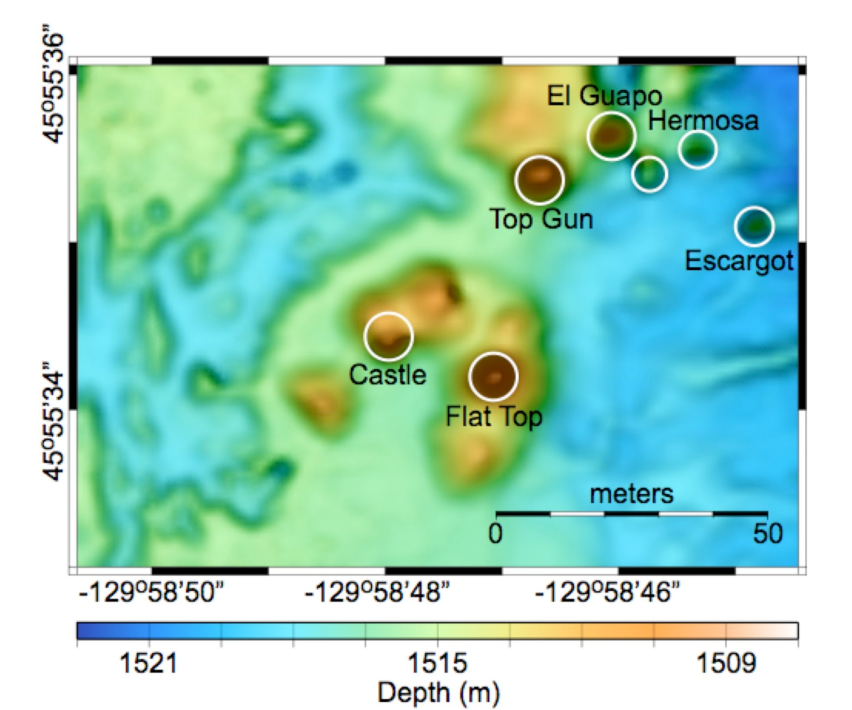
\includegraphics[scale=0.35]{figs/vents.pdf}}\\
  \subfloat[\small An illustration of our domain]{\label{fig:ex:graph}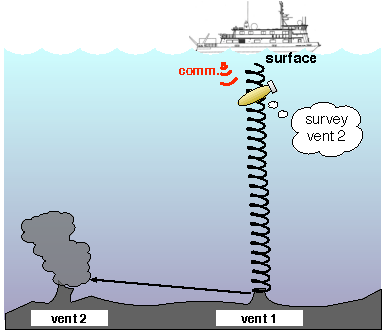
\includegraphics[width=0.51\columnwidth]{figs/auv_example}}
  \hfill \subfloat[\small Initial  problem]{\label{fig:ex:init}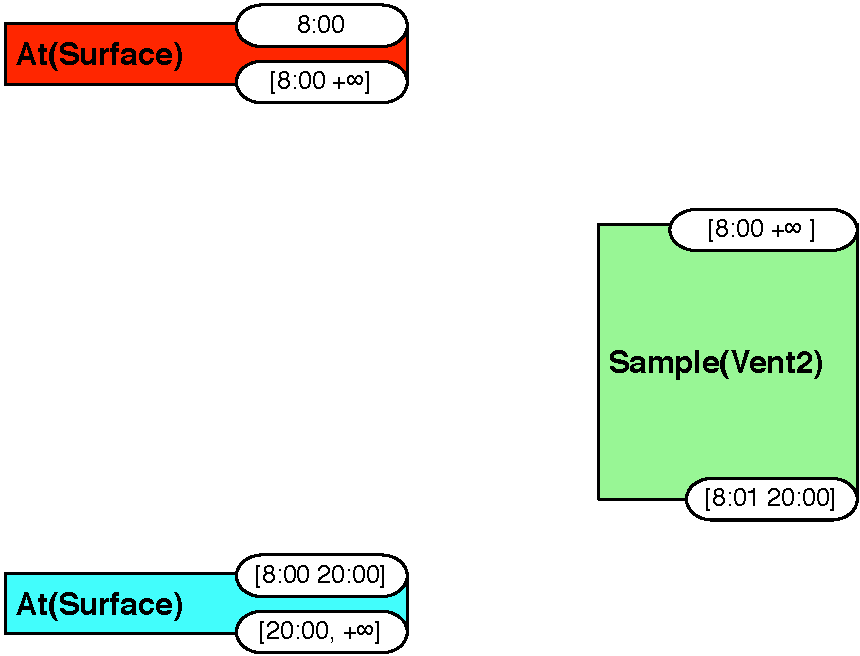
\includegraphics[width=0.47\columnwidth]{figs/example_initial}}
  \caption{\small{\ref{fig:ex:axial} shows bathymetry of actual vent
      sites off the coast of Oregon. A description of a hydrotermal
      vent problem with an illustration of the domain
      (\ref{fig:ex:graph}) along with the initial partial plan for
      this probelem (\ref{fig:ex:init}). In this domain our AUV is
      initially at {\em Surface} at 8am, he wants to survey {\em vent
        2} which is active before noon and needs to be back at {\em
        Surface} before the end of its mission at 8pm (noted 20:00
      here).}}
\label{fig:Example}
\end{figure}

However, an issue with finding a balanced approach is deciding whether
it starts to starts its action as early as possible -- which we will
call proactive \fcomment{Need to replace least-commitment by
  ``proactive''}
-- or wait until the action should necessary start --
called later deferred\fcomment{similarly rename EST as ``deferred''}. 
makeThere is a clear difference between the two approaches
 but when should, for example, the shopping agent wait
or start early ? Lets demonstrate an ideal scenario where the shopping
agent balances both approaches illustrated in Figure \ref{fig:Example}. 

The agent, waking up at 8 AM, {\em wants} to buy an apple
and {\em needs} to be home by 8 PM. The agent then leaves as early as
possible to start shopping. Considering that that it takes 20 minutes
to half an hour to go from Home to the Clothing Shop, 10 to 15 minutes
to go from the Clothing shop to Grocery and 5 to 10 minutes in order
to buy an apple, a general plan solution is presented in  Figure
\ref{fig:ex:plan}. The plan presented here is partially instantiated
giving the agent the freedom to decide when to start an action within
the valid boundary of the solution. The agent can then for example go
early on buy its apple so he is sure to have it as early as possible. Conversely,
the agent may decide to walk around and fo window shopping throughout
the rest of the day as there is no hurry yet. By 7pm though, it should
eventually leave so it can arrive back home by 8pm. In this scenario,
we see that agent did alternate between deciding to execute actions
early or procrastinate depending on the the nature of the action it
need to take next or more accurately the nature of the objectives 
related to this action. Indeed, the agent was proactive on leaving his 
house as it was related to him {\em
  wanting}  an apple, on the other hand he just {\em needed} to get
back home by 8 PM allowing him to procrastinate at the grocery 
store. By doing so he will be around in case his wife is calling him
to buy extract things before he gets back home. 

% \fcomment{Need a figure that shows the plan somehow ... this can be
%   refined as we go along for illustrating proactive vs deferred}

\begin{figure}
  \centering
  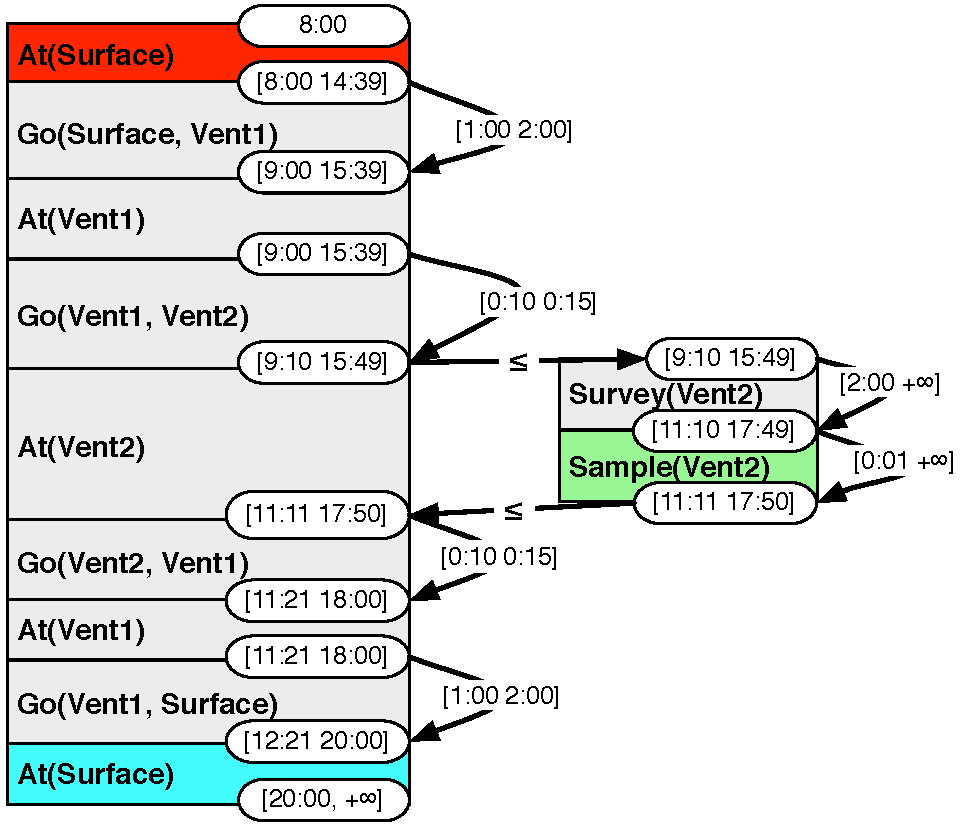
\includegraphics[width=0.8\columnwidth]{figs/example_plan}
  \caption{The flexible plan solution of our domain in
    Fig. \ref{fig:Example}}
  \label{fig:ex:plan}
\end{figure}

While this example may appear academic at first, it reflects situations
er have seen within embedded agent execution in our domain. Indeed, we
do daily operations wehere our AUV is deployed and scientists can
remotely send new objectives as the mission goes along to the vehicle
as they see new area of interrest. At the same time the vehicle has
also operational objectives such as going to a place where its
recovery will be easier for operators. This gives a similar
distinction between the science objectives and operation
objectives. Similarly to our shopping agent we do not really want the
AUV to get back to recovery area too early as a new science goal could
be sent to him which in turns would rather be fulfilled as early as
possible.

This paper discusses the problem of dispatching when trying to execute
a plan. In particular, dispatching in a dynamic environment where the
plan is known to change either by uncontrollable events or external
requests with new directives. External requests  can occur
at any time which make them in essence uncontrollable events.
Specifically, we focus on how these new requests, coming from the
external world, will affect the way we dispatch the plan, rather than
how they will be integrated into the plan or any part of the planning
process.  The reason for our separation from planning is that
oftentimes planning and executing are split up into two different
jobs. Where a robotic agent is give an already created plan, and it
must then choose how to execute that plan. Therefore, our focus is on
how to dispatch a plan after it has already been created, while
understanding that the plan may still change in the near future.

The approach we have taken on dispatching looks at the token level of a plan,
specifically at the externally requested tokens which we define as goals.
Because they are requested by an external person with the intent of being 
completed, they have a high priority. In contrast, there are tokens that only describe the
evolution of a timeline, which we define as non-goals. In order to keep the plan 
valid, the agent is obligated to complete the non-goals, but there is no rush. Thus, the
non-goals have a low priority. Therefore, we want to complete the goals
as early as possible in order to give adequate time for the possibility of new
goals, and complete the non-goals as they become necessary for the validity of the plan. 
Some may argue that finishing the goals early doesn't guarantee that
there will be enough time for new goals, however, that is an issue with planning, 
and our concern is with dispatching.


%%% Local Variables: 
%%% mode: latex
%%% TeX-master: "aaai13"
%%% End: 
